\begin{frame}[allowframebreaks]{Hierarchical ViT: Swin Transformer}
    \begin{figure}
        \centering
        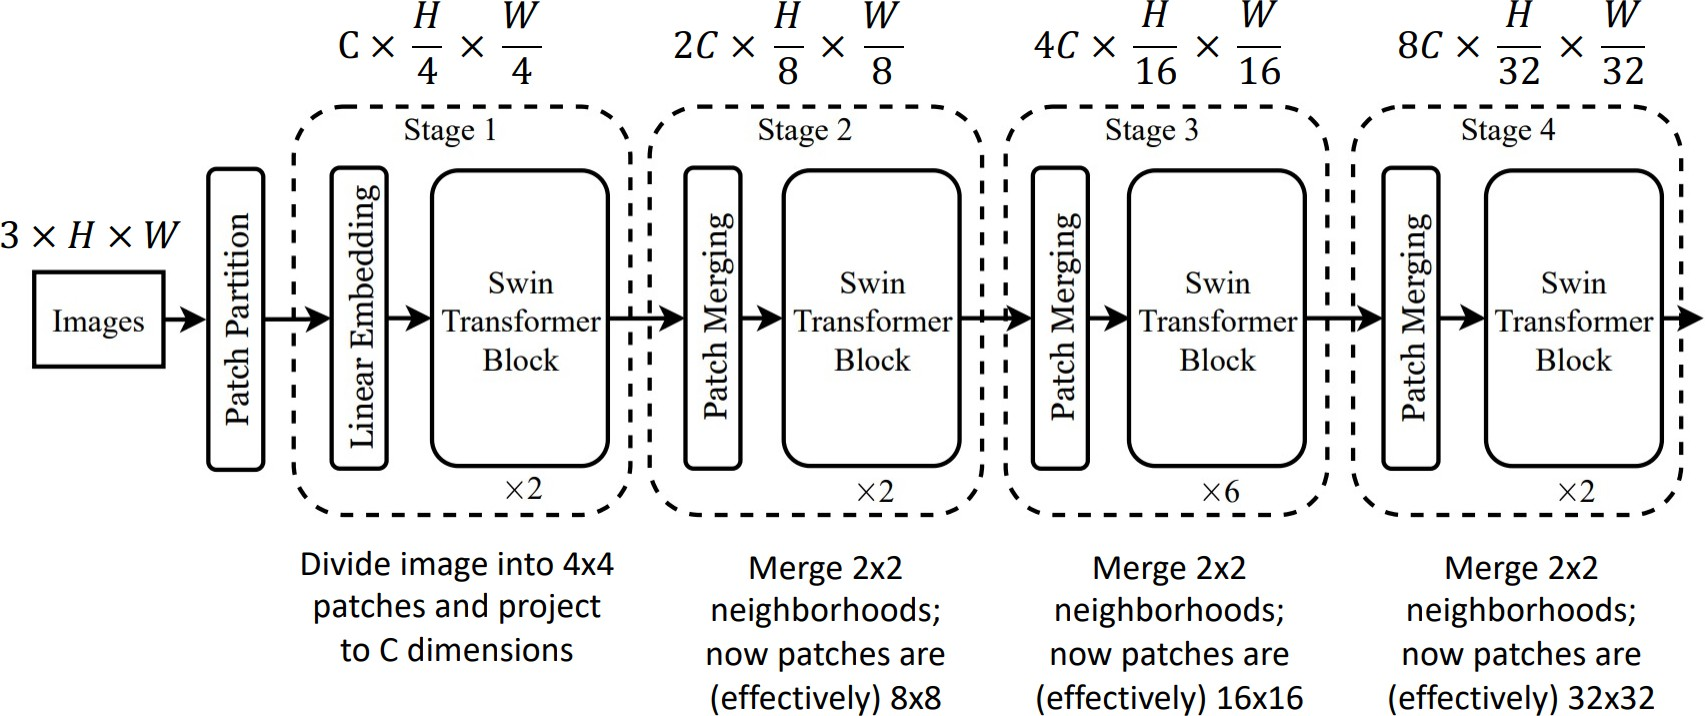
\includegraphics[width=\linewidth,height=0.9\textheight,keepaspectratio]{images/vit/slide_69_1_img.jpg}
    \end{figure}

    \framebreak
    \begin{itemize}
        \item Swin Transformer introduces windowed self-attention with shifting windows, merging tokens akin to pooling.\footnote{\url{https://arxiv.org/abs/2103.14030}}
        \item Builds a pyramid representation, enabling linear compute complexity and high performance on detection/segmentation (e.g. 58.7 COCO box AP).
        \item Hierarchical design allows for multi-scale feature extraction, similar to CNNs.
    \end{itemize}

    \framebreak

    \begin{figure}
        \centering
        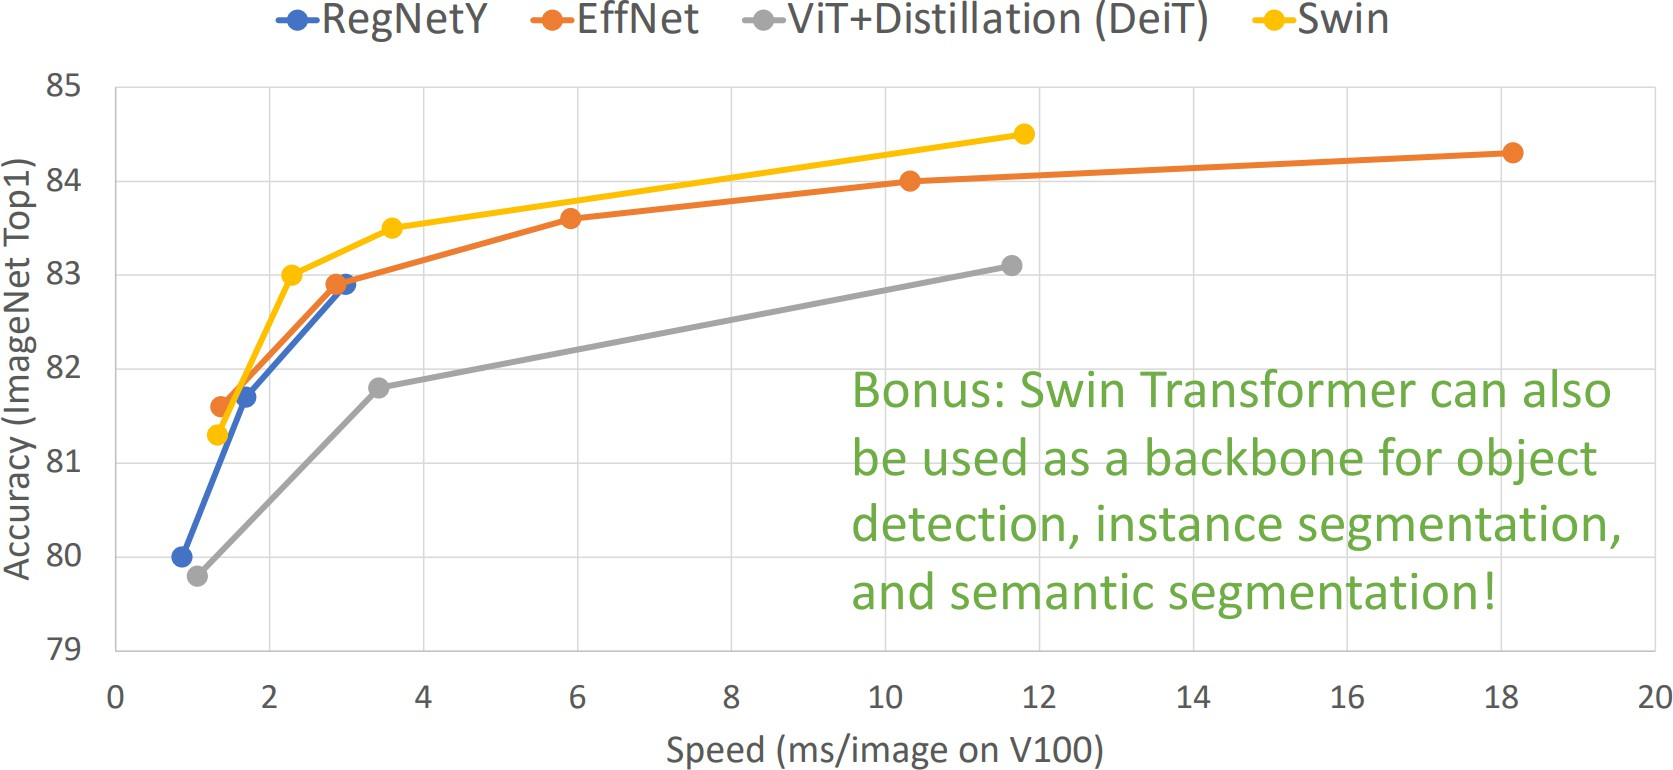
\includegraphics[width=\linewidth,height=0.9\textheight,keepaspectratio]{images/vit/slide_70_1_img.jpg}
        \footnote{Liu et al, “Swin Transformer: Hierarchical Vision Transformer using Shifted Windows”, CVPR 2021}
    \end{figure}
\end{frame}

\begin{frame}[allowframebreaks]{Other Hierarchical Vision Transformers}
    \begin{figure}
        \centering
        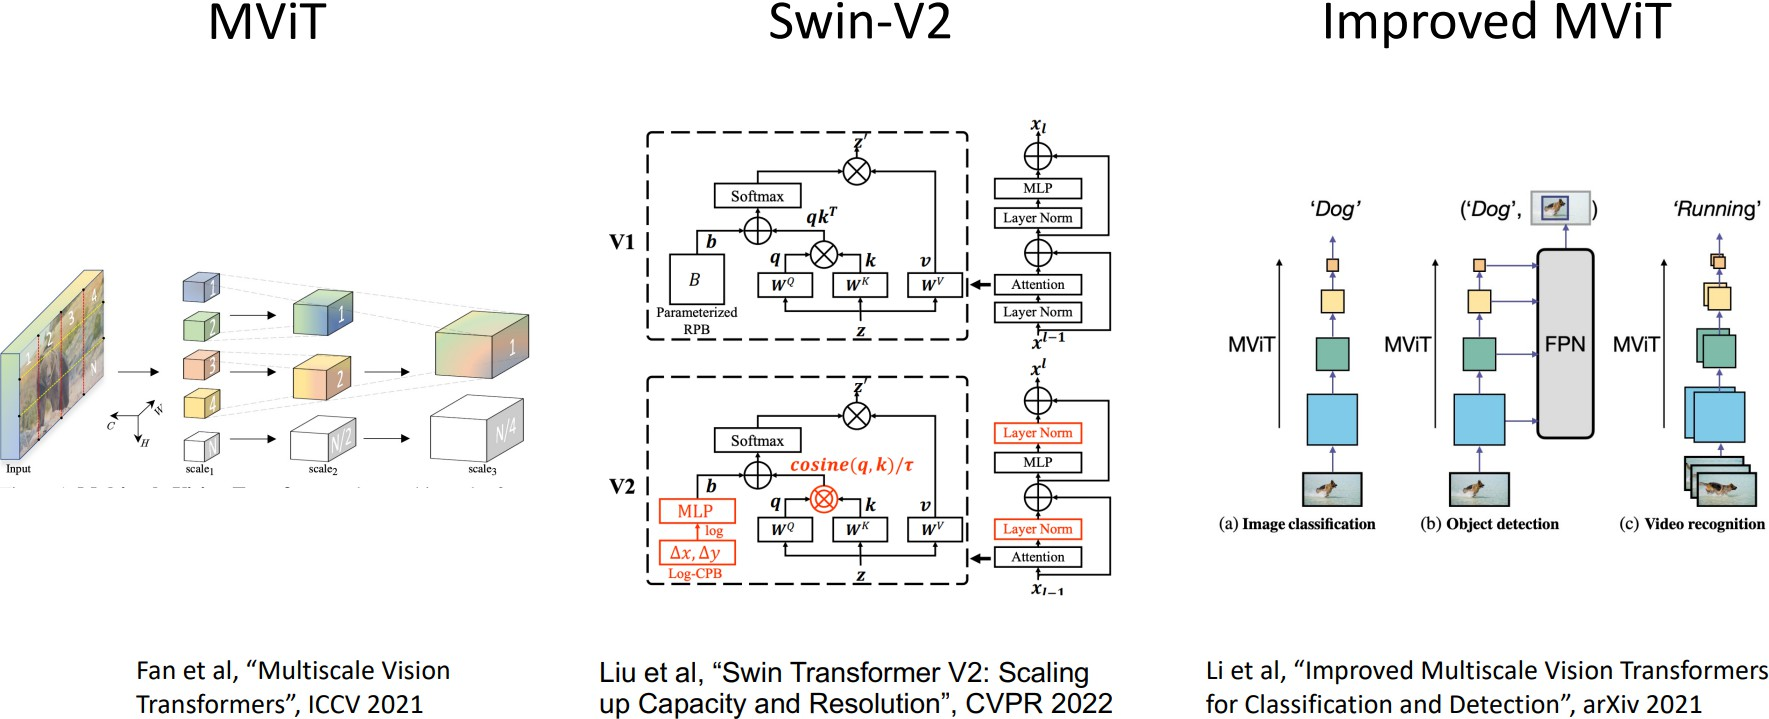
\includegraphics[width=\linewidth,height=0.9\textheight,keepaspectratio]{images/vit/slide_71_1_img.jpg}
    \end{figure}
\end{frame}